\section{Beyond ECE: Rank-Safe Recalibration, Transfer, Coverage, and Robustness}
\label{sec:extended}

This section adds analyses that sharpen the paper's central message---that ECG foundation
models are strong rankers but unreliable probability estimators---and turns the
``calibration can hurt AUROC'' observation into a method. All results use the same fixed,
patient-split probability caches as Section~\ref{sec:results} (real data only).

\subsection{Beyond ECE: Proper Scores and Calibration Curves}
\label{sec:extended-metrics}

ECE is neither a proper scoring rule nor binning-invariant, so we additionally report
adaptive (equal-mass) ECE, negative log-likelihood (NLL, proper), and the Cox calibration
\emph{slope} (ideal $1$) and \emph{intercept} (ideal $0$), aligning with clinical
prediction-model reporting (TRIPOD+AI). Table~\ref{tab:extended-metrics} confirms the ECE
picture is not a binning artefact: PTB-XL has the worst NLL (0.49 mean) and the lowest
calibration slope (0.40), i.e.\ the most over-confident logits, while CODE-15\% and CPSC2018
slopes approach 1. Calibration slopes below 1 with negative intercepts---present for every
foundation model on PTB-XL---are the signature of over-confidence that recalibration
corrects.

\begin{table}[t]
\centering
\caption{Extended calibration metrics beyond ECE (macro over valid classes, test split), averaged per dataset. NLL = negative log-likelihood; calibration slope (ideal $=1$) and intercept (ideal $=0$) from Cox recalibration of labels on logits. Slopes far below 1 and negative intercepts indicate systematic over-confidence that worsens on PTB-XL.}
\label{tab:extended-metrics}
\small
\begin{tabular}{lccccc}
\toprule
Dataset & ECE & adaptive ECE & NLL & cal.\ slope & cal.\ intercept \\
\midrule
  PTB-XL & 0.097 & 0.093 & 0.495 & 0.446 & -0.591 \\
  CODE-15\% & 0.023 & 0.022 & 0.166 & 0.413 & -1.401 \\
  CPSC2018 & 0.032 & 0.030 & 0.234 & 0.651 & -0.514 \\
  MIMIC-IV-ECG & 0.074 & 0.072 & 0.383 & 0.423 & -0.233 \\
\bottomrule
\end{tabular}
\end{table}

\subsection{RankSafe-Cal: Recalibration that Preserves Ranking}
\label{sec:ranksafe}

Unconstrained isotonic regression achieves the lowest ECE but, being only weakly monotone,
can merge ties and reduce AUROC (up to $0.032$ per class on PTB-XL, mean $-0.011$). We
introduce \textbf{RankSafe-Cal}, which makes the discrimination cost an explicit constraint.

\begin{algorithm}[t]
\caption{RankSafe-Cal (per class)}
\label{alg:ranksafe}
\begin{algorithmic}[1]
\Require calibration probs/labels $(p_c,y_c)$, test probs $p_t$, tolerance $\epsilon$,
  candidates $\mathcal{M}=\{$Platt, temperature, isotonic$\}$
\State split $(p_c,y_c)$ into fit/select halves $(p_f,y_f),(p_s,y_s)$
\For{each $m\in\mathcal{M}$}
  \State fit $m$ on $(p_f,y_f)$; $\;\hat p_s \gets m(p_s)$
  \State $\Delta\mathrm{AUROC}_m \gets \mathrm{AUROC}(y_s,p_s)-\mathrm{AUROC}(y_s,\hat p_s)$ \Comment{out-of-sample}
  \State $\mathrm{ECE}_m \gets \mathrm{ECE}(y_s,\hat p_s)$
\EndFor
\State $\mathcal{S}\gets\{m:\Delta\mathrm{AUROC}_m\le\epsilon\}$ \Comment{Platt/temperature are strictly monotone $\Rightarrow \Delta\mathrm{AUROC}\approx0$}
\State $m^\star \gets \arg\min_{m\in\mathcal{S}} \mathrm{ECE}_m$ \quad(fallback: $\arg\min_m \Delta\mathrm{AUROC}_m$)
\State refit $m^\star$ on full $(p_c,y_c)$; \Return $m^\star(p_t)$
\end{algorithmic}
\end{algorithm}

\paragraph{Ranking-preservation argument.}
A strictly increasing transform $g$ leaves the ROC curve---and hence AUROC---unchanged,
because it preserves the ordering of scores used to sweep thresholds. Platt scaling
(logistic, positive slope) and temperature scaling ($T>0$) are strictly increasing, so their
per-class AUROC loss is $0$ in the population; isotonic is only weakly monotone and can lose
AUROC. RankSafe-Cal certifies $\Delta\mathrm{AUROC}\le\epsilon$ on held-out calibration data,
so it also rejects the rare case where a noisy Platt fit inverts on a low-prevalence class.

Table~\ref{tab:ranksafe} and Figure~\ref{fig:ranksafe} show the payoff. On PTB-XL,
RankSafe-Cal ($\epsilon{=}0.01$) cuts mean ECE from $0.097$ to $0.054$ (vs.\ isotonic
$0.046$) while reducing the AUROC loss roughly six-fold ($+0.0018$ vs.\ isotonic $+0.0108$;
worst-class $0.018$ vs.\ $0.032$). On MIMIC-IV-ECG it \emph{beats} unconstrained isotonic on
both axes (ECE $0.043$ vs.\ $0.045$; AUROC loss $+0.0027$ vs.\ $+0.0108$). RankSafe-Cal thus
recovers the large majority of isotonic's calibration benefit at a small, bounded, and often
negligible discrimination cost---the recommended default when the model's ranking is itself
clinically used (e.g.\ triage ordering).

\begin{table}[t]
\centering
\caption{RankSafe-Cal vs.\ baselines (mean over models per dataset). RankSafe-Cal selects, per class, the lowest-ECE recalibrator whose \emph{out-of-sample} AUROC loss is within $\epsilon{=}0.01$ (certified on a held-out half of the calibration split). It recovers most of unconstrained isotonic's ECE reduction at a fraction of the AUROC cost. Max class loss = worst per-class test AUROC drop vs.\ raw.}
\label{tab:ranksafe}
\small
\begin{tabular}{llccc}
\toprule
Dataset & Method & ECE $\downarrow$ & AUROC loss $\downarrow$ & max class loss $\downarrow$ \\
\midrule
  PTB-XL & Raw & 0.097 & +0.0000 & 0.000 \\
   & Platt & 0.057 & +0.0000 & 0.000 \\
   & Temperature & 0.078 & +0.0000 & 0.000 \\
   & Isotonic (unconstr.) & 0.046 & +0.0108 & 0.032 \\
   & \textbf{RankSafe-Cal} & 0.054 & +0.0018 & 0.018 \\
  \midrule
  CODE-15\% & Raw & 0.023 & +0.0000 & 0.000 \\
   & Platt & 0.016 & +0.0178 & 0.225 \\
   & Temperature & 0.018 & +0.0002 & 0.004 \\
   & Isotonic (unconstr.) & 0.013 & +0.0078 & 0.109 \\
   & \textbf{RankSafe-Cal} & 0.014 & +0.0094 & 0.225 \\
  \midrule
  CPSC2018 & Raw & 0.032 & +0.0000 & 0.000 \\
   & Platt & 0.027 & +0.0000 & 0.000 \\
   & Temperature & 0.029 & +0.0000 & 0.002 \\
   & Isotonic (unconstr.) & 0.020 & +0.0075 & 0.059 \\
   & \textbf{RankSafe-Cal} & 0.024 & +0.0009 & 0.008 \\
  \midrule
  MIMIC-IV-ECG & Raw & 0.074 & +0.0000 & 0.000 \\
   & Platt & 0.042 & +0.0000 & 0.000 \\
   & Temperature & 0.068 & -0.0001 & 0.000 \\
   & Isotonic (unconstr.) & 0.044 & +0.0108 & 0.049 \\
   & \textbf{RankSafe-Cal} & 0.043 & +0.0027 & 0.040 \\
\bottomrule
\end{tabular}
\end{table}

\begin{figure}[t]
  \centering
  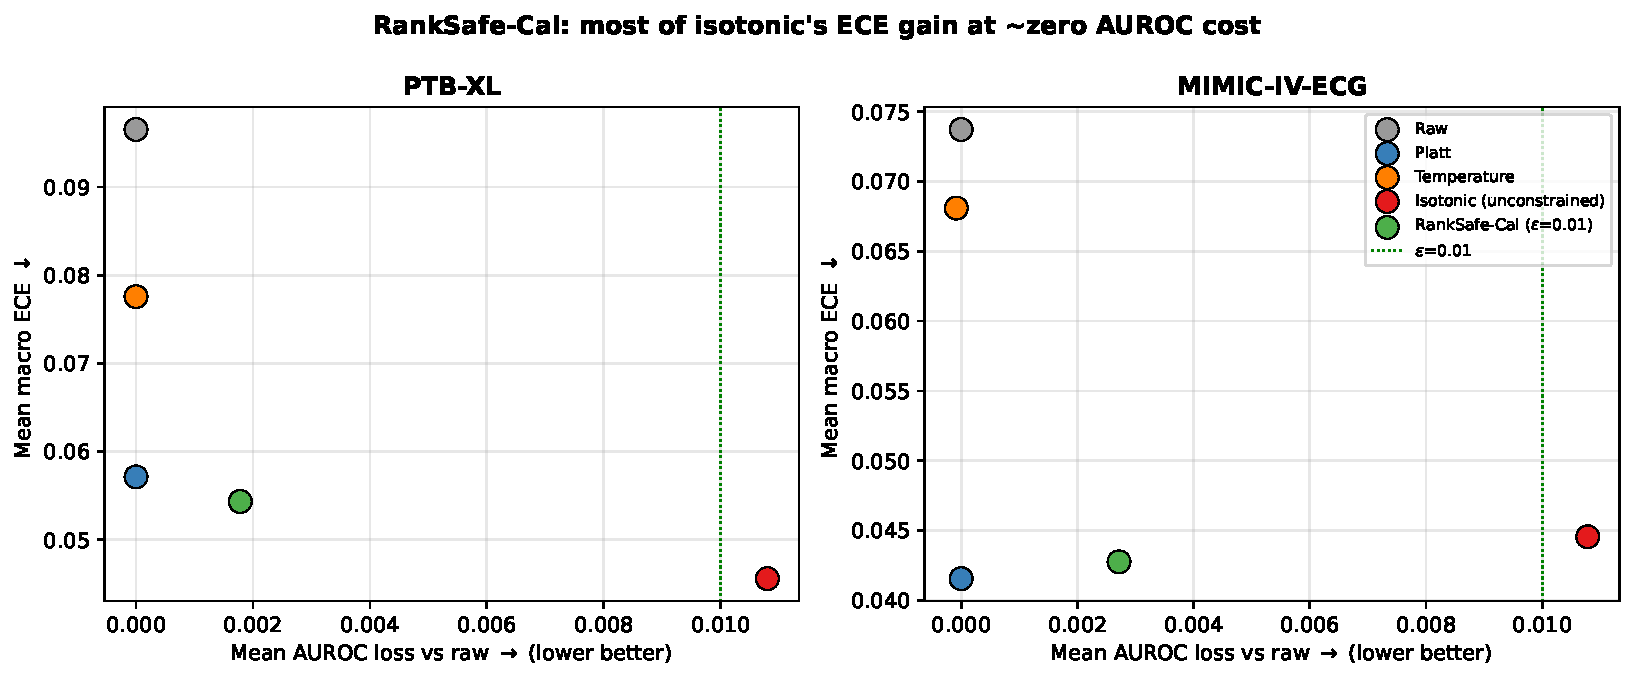
\includegraphics[width=0.92\linewidth]{figures/fig_ranksafe.pdf}
  \caption{RankSafe-Cal vs.\ baselines on the two multi-morbidity datasets (mean over models).
    RankSafe-Cal sits near isotonic's ECE but at the green AUROC-loss tolerance, whereas
    unconstrained isotonic pays a larger ranking cost.}
  \label{fig:ranksafe}
\end{figure}

\subsection{Cross-Dataset Calibration Transfer}
\label{sec:extended-transfer}

Is recalibration portable across cohorts? We fit a calibrator on a \emph{source} dataset's
calibration split and apply it to a \emph{target} dataset's test split, for diagnostic
endpoints shared across datasets (MI: PTB-XL$\leftrightarrow$MIMIC; AF and RBBB across
CODE-15\%/CPSC2018/MIMIC; Normal across all). Table~\ref{tab:transfer} reports, per endpoint,
raw vs.\ locally-recalibrated vs.\ transferred ECE. Transfer succeeds (transferred ECE within
25\% of in-domain and below raw) in only $42\%$ of MI pairs, $41\%$ of RBBB, $28\%$ of AF, and
$9\%$ of Normal pairs. Calibration is therefore \textbf{largely deployment-context-specific}:
a calibrator learned on one cohort frequently fails to transfer, and the degree of failure is
endpoint-dependent (worst for the high-prevalence Normal class). This strengthens the
local-audit recommendation---recalibration should be re-fit on data representative of the
deployment population rather than imported from a benchmark.

\begin{table}[t]
\centering
\caption{Cross-dataset calibration \emph{transfer} (isotonic, one-vs-rest). A calibrator fit on a source dataset's calibration split is applied to a target dataset's test split. ECE values are means over (model, source$\to$target) pairs. Transfer success = transferred ECE within 25\% of the in-domain recalibrated ECE and below raw. Calibration transfers partially and endpoint-dependently---it does not fully substitute for local recalibration.}
\label{tab:transfer}
\small
\begin{tabular}{lcccccc}
\toprule
Endpoint & $n$ pairs & raw ECE & in-dom.\ ECE & transf.\ ECE & success & mean $\Delta$AUROC \\
\midrule
  MI (PTB-XL$\leftrightarrow$MIMIC) & 12 & 0.101 & 0.055 & 0.061 & 42\% & -0.008 \\
  AF (CODE/CPSC/MIMIC) & 32 & 0.039 & 0.026 & 0.040 & 28\% & -0.021 \\
  Normal (all) & 66 & 0.083 & 0.045 & 0.133 & 9\% & -0.025 \\
  RBBB (CODE/CPSC/MIMIC) & 32 & 0.032 & 0.020 & 0.036 & 41\% & -0.006 \\
\bottomrule
\end{tabular}
\end{table}

\begin{figure}[t]
  \centering
  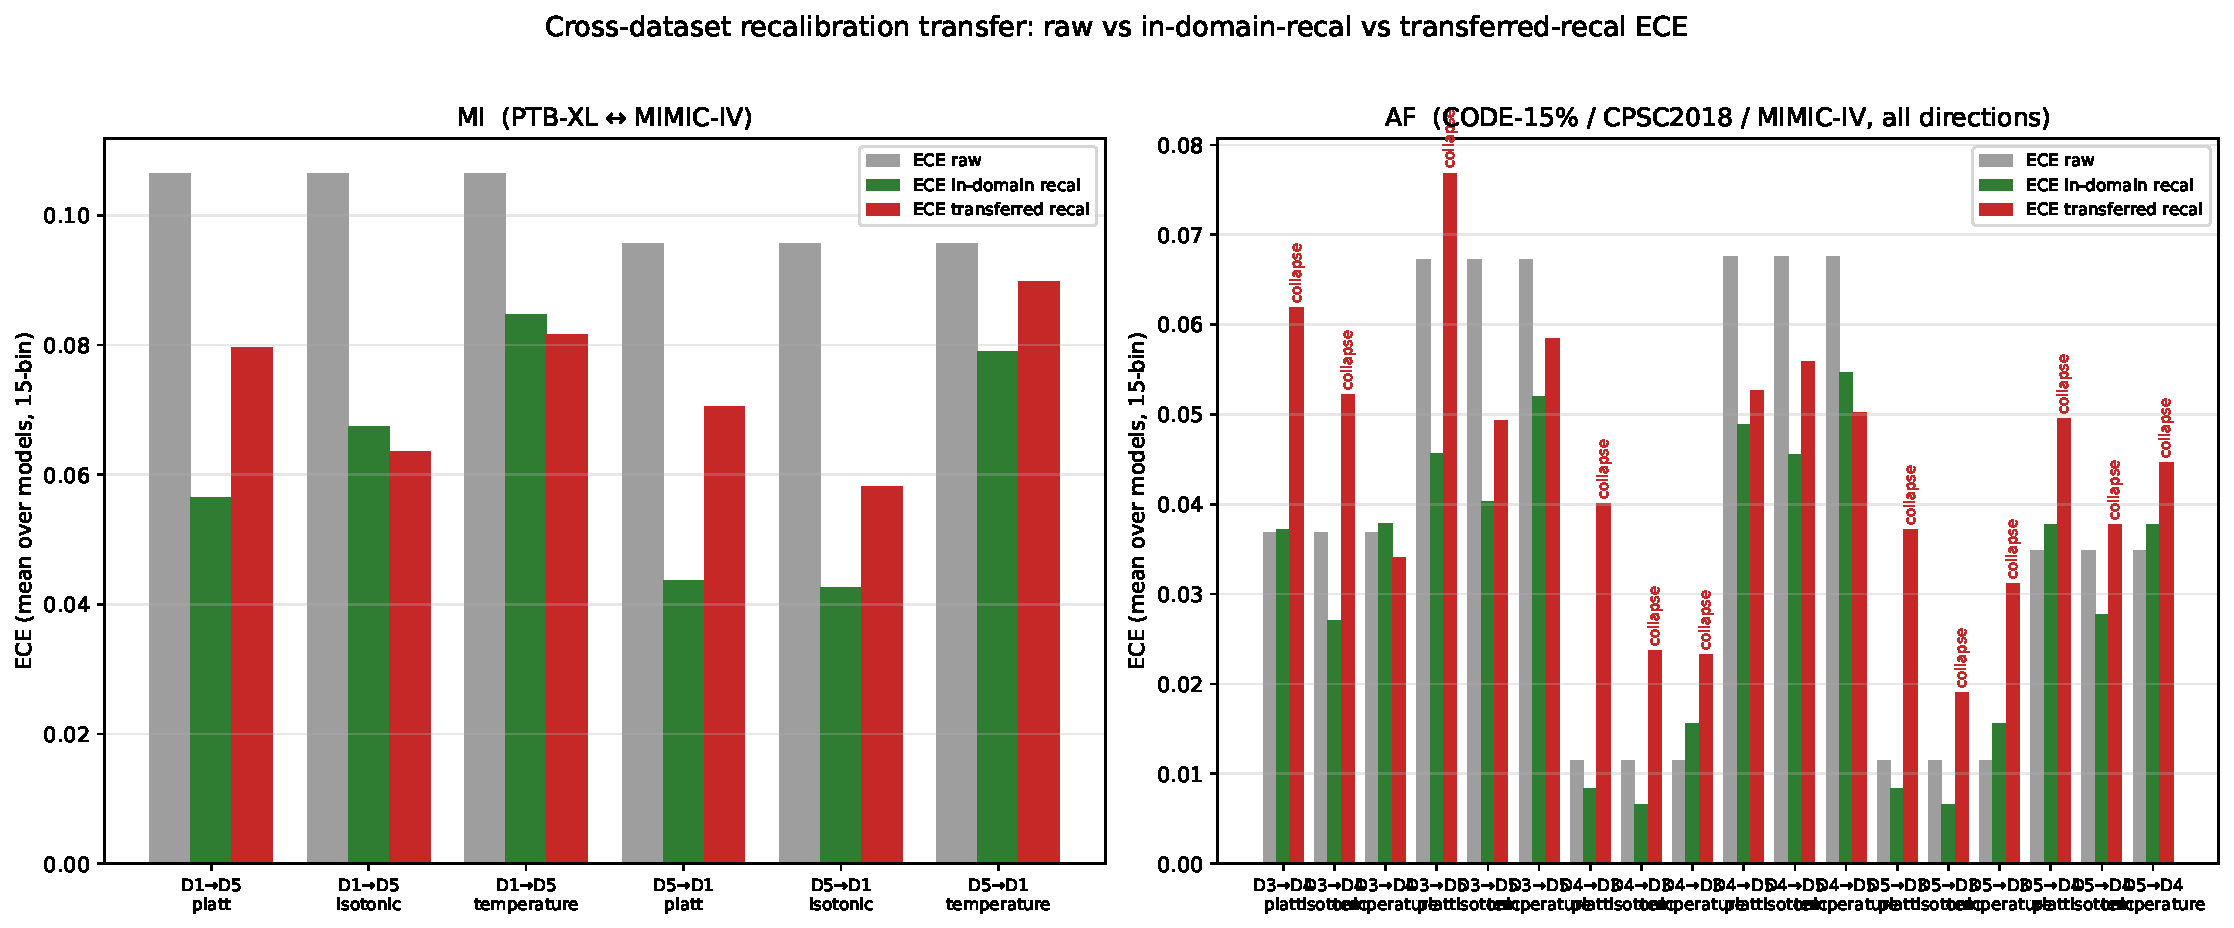
\includegraphics[width=0.96\linewidth]{figures/fig_transfer.pdf}
  \caption{Cross-dataset calibration transfer (isotonic). Transferred recalibration (rightmost
    bars) often fails to match in-domain recalibration and sometimes exceeds the raw ECE
    (collapse), especially for AF and Normal under dataset shift.}
  \label{fig:transfer}
\end{figure}

\subsection{Conformal Prediction: Coverage Guarantees}
\label{sec:extended-conformal}

Recalibration improves probability \emph{reliability} but offers no finite-sample guarantee.
We add split-conformal prediction (one-vs-rest) for MI, AF, and Normal, building conformal
sets from calibration scores at target coverage $90\%$. Table~\ref{tab:conformal} shows
empirical coverage meets the target for every method and endpoint (the distribution-free
guarantee holds), while recalibration affects only \emph{efficiency}: Platt yields the
smallest sets, isotonic the largest (its heavy ties inflate set size), and temperature
scaling---being order-preserving---produces conformal sets identical to raw. Class-conditional
coverage is asymmetric for rare endpoints (true negatives over-covered, true positives
under-covered), an important caveat for minority cardiac findings. Conformal prediction is
thus complementary to calibration: calibration makes the scalar probability trustworthy;
conformal turns it into a set with a provable miscoverage bound.

\begin{table}[t]
\centering
\caption{Split-conformal prediction (one-vs-rest, target coverage $1-\alpha=0.90$), mean over models/datasets. Empirical coverage meets the target for all methods (finite-sample guarantee); recalibration mainly affects set-size efficiency. Temperature scaling is order-preserving so its conformal sets are identical to raw.}
\label{tab:conformal}
\small
\begin{tabular}{llcc}
\toprule
Endpoint & Method & coverage & avg.\ set size \\
\midrule
  MI & raw & 0.900 & 1.209 \\
   & platt & 0.900 & 1.183 \\
   & isotonic & 0.900 & 1.203 \\
   & temperature & 0.900 & 1.209 \\
  \midrule
  AF & raw & 0.900 & 0.990 \\
   & platt & 0.900 & 0.980 \\
   & isotonic & 0.900 & 1.003 \\
   & temperature & 0.900 & 0.990 \\
  \midrule
  NORM & raw & 0.900 & 1.267 \\
   & platt & 0.900 & 1.258 \\
   & isotonic & 0.900 & 1.327 \\
   & temperature & 0.900 & 1.267 \\
\bottomrule
\end{tabular}
\end{table}

\begin{figure}[t]
  \centering
  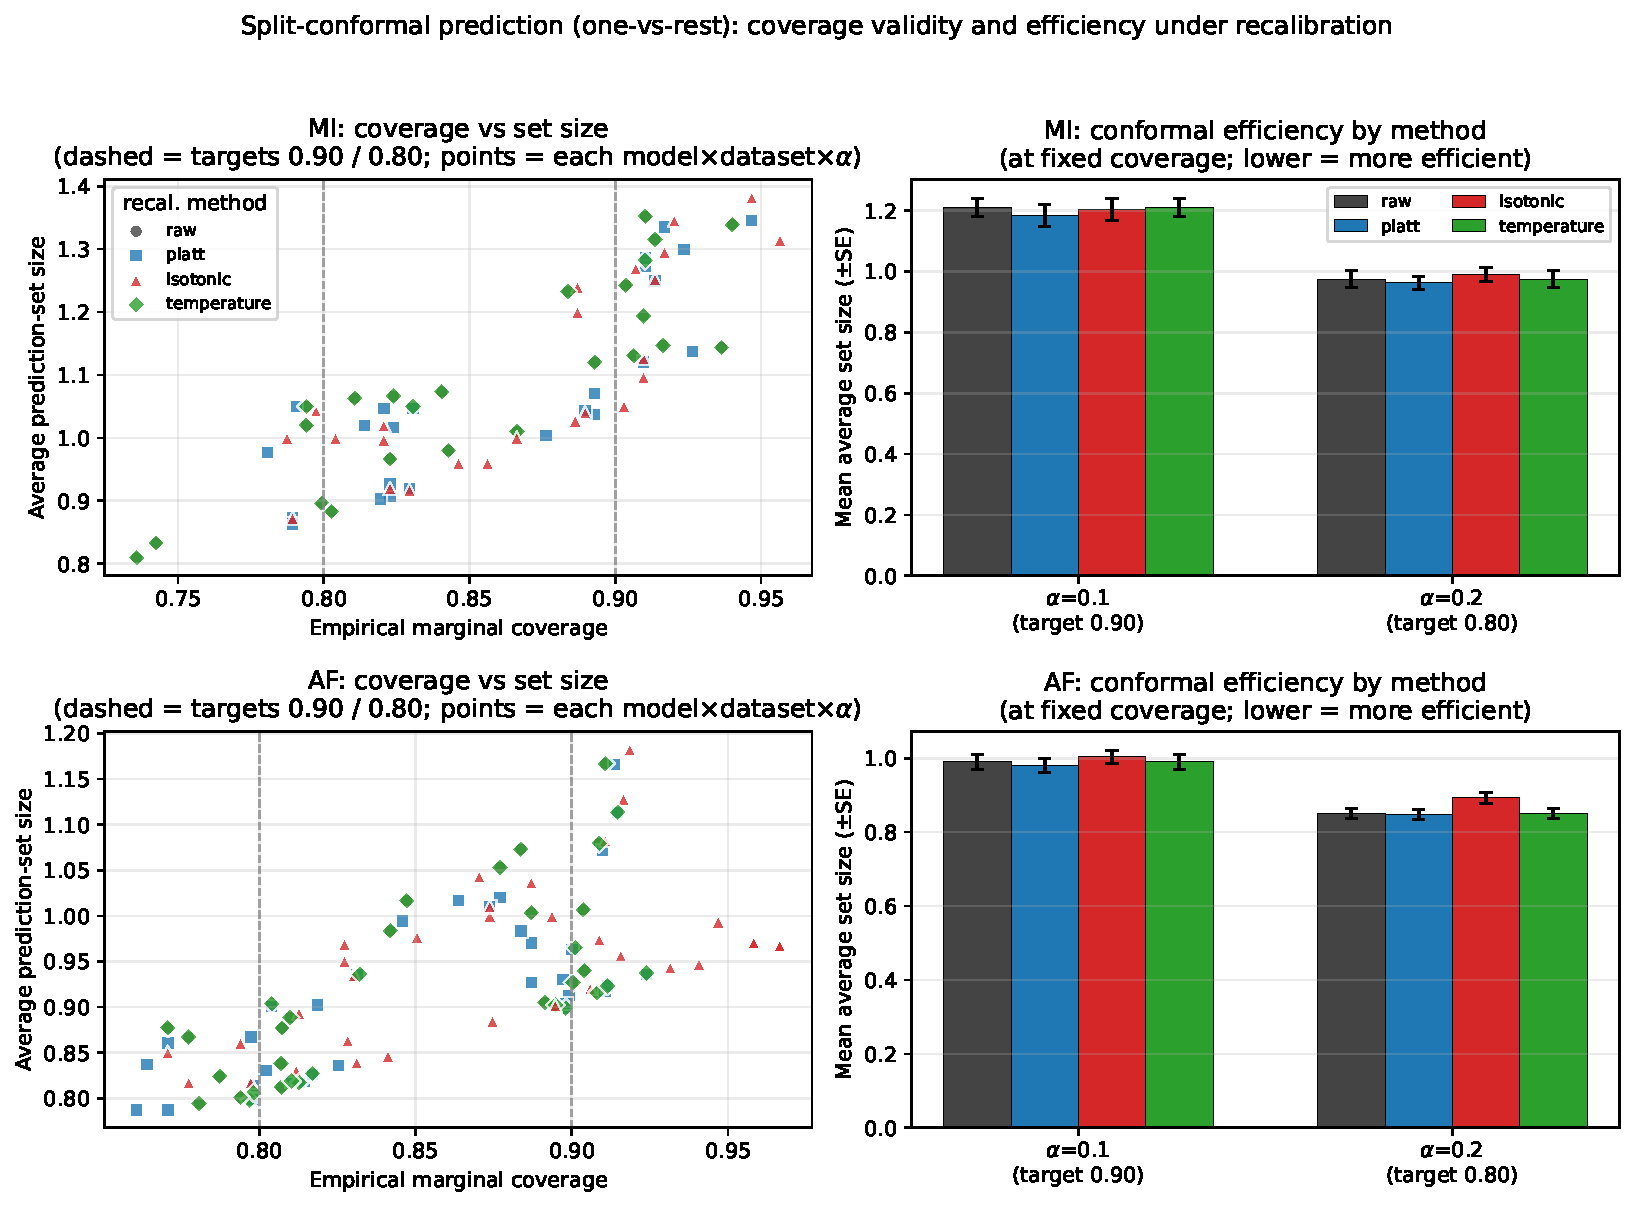
\includegraphics[width=0.96\linewidth]{figures/fig_conformal.pdf}
  \caption{Split-conformal prediction for the MI and AF endpoints: empirical coverage vs.\
    average set size by method. All methods attain target coverage; Platt is most efficient.}
  \label{fig:conformal}
\end{figure}

\subsection{Expanded Clinical Decision-Curve Analysis}
\label{sec:extended-dca}

We extend decision-curve analysis from a single curve to MI (PTB-XL, MIMIC-IV-ECG) and AF
(CODE-15\%, CPSC2018, MIMIC-IV-ECG) for all models, integrating net benefit over clinically
plausible threshold ranges (Figures~\ref{fig:dca-mi}--\ref{fig:dca-af}). Every model delivers
positive integrated net benefit above treat-all at MI thresholds (e.g.\ ST-MEM PTB-XL
$+0.027$; net benefit $+0.046$ at $t{=}0.15$), confirming that FM \emph{rankings} already
support useful decisions. For the rarer AF endpoint, integrated net benefit above treat-all is
large (e.g.\ $+0.19$ on CODE-15\%) because indiscriminate treat-all is costly at low
prevalence. Recalibration leaves integrated net benefit essentially unchanged (rank-preserving
methods cannot alter it, and isotonic changes it only marginally), but it is what makes the
\emph{probability} attached to each decision trustworthy---necessary when the numeric risk is
communicated or combined across models.

\begin{figure}[t]
  \centering
  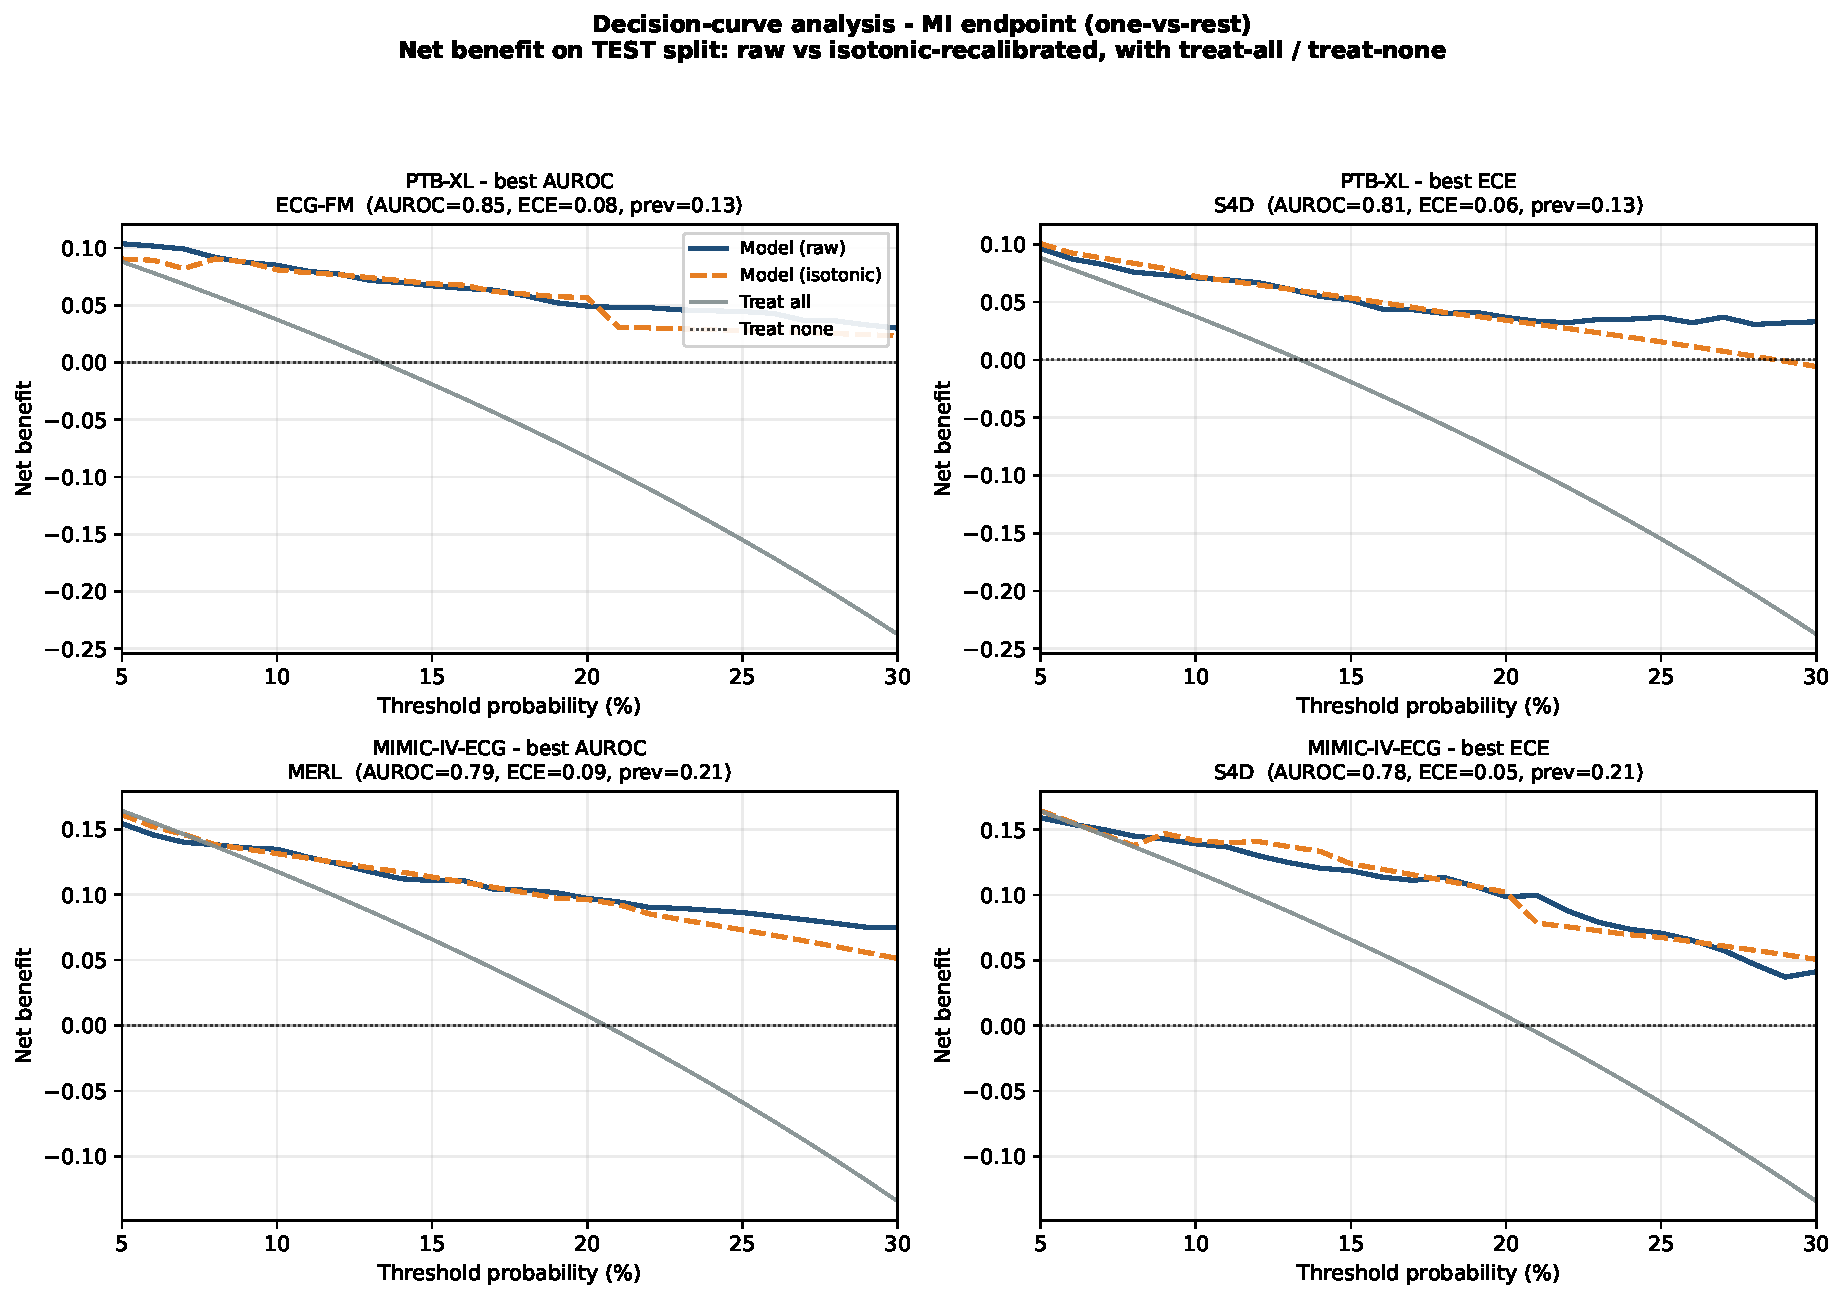
\includegraphics[width=0.96\linewidth]{figures/fig_dca_mi.pdf}
  \caption{Decision-curve analysis for MI on PTB-XL and MIMIC-IV-ECG, raw vs.\ isotonic, with
    treat-all/treat-none references.}
  \label{fig:dca-mi}
\end{figure}

\begin{figure}[t]
  \centering
  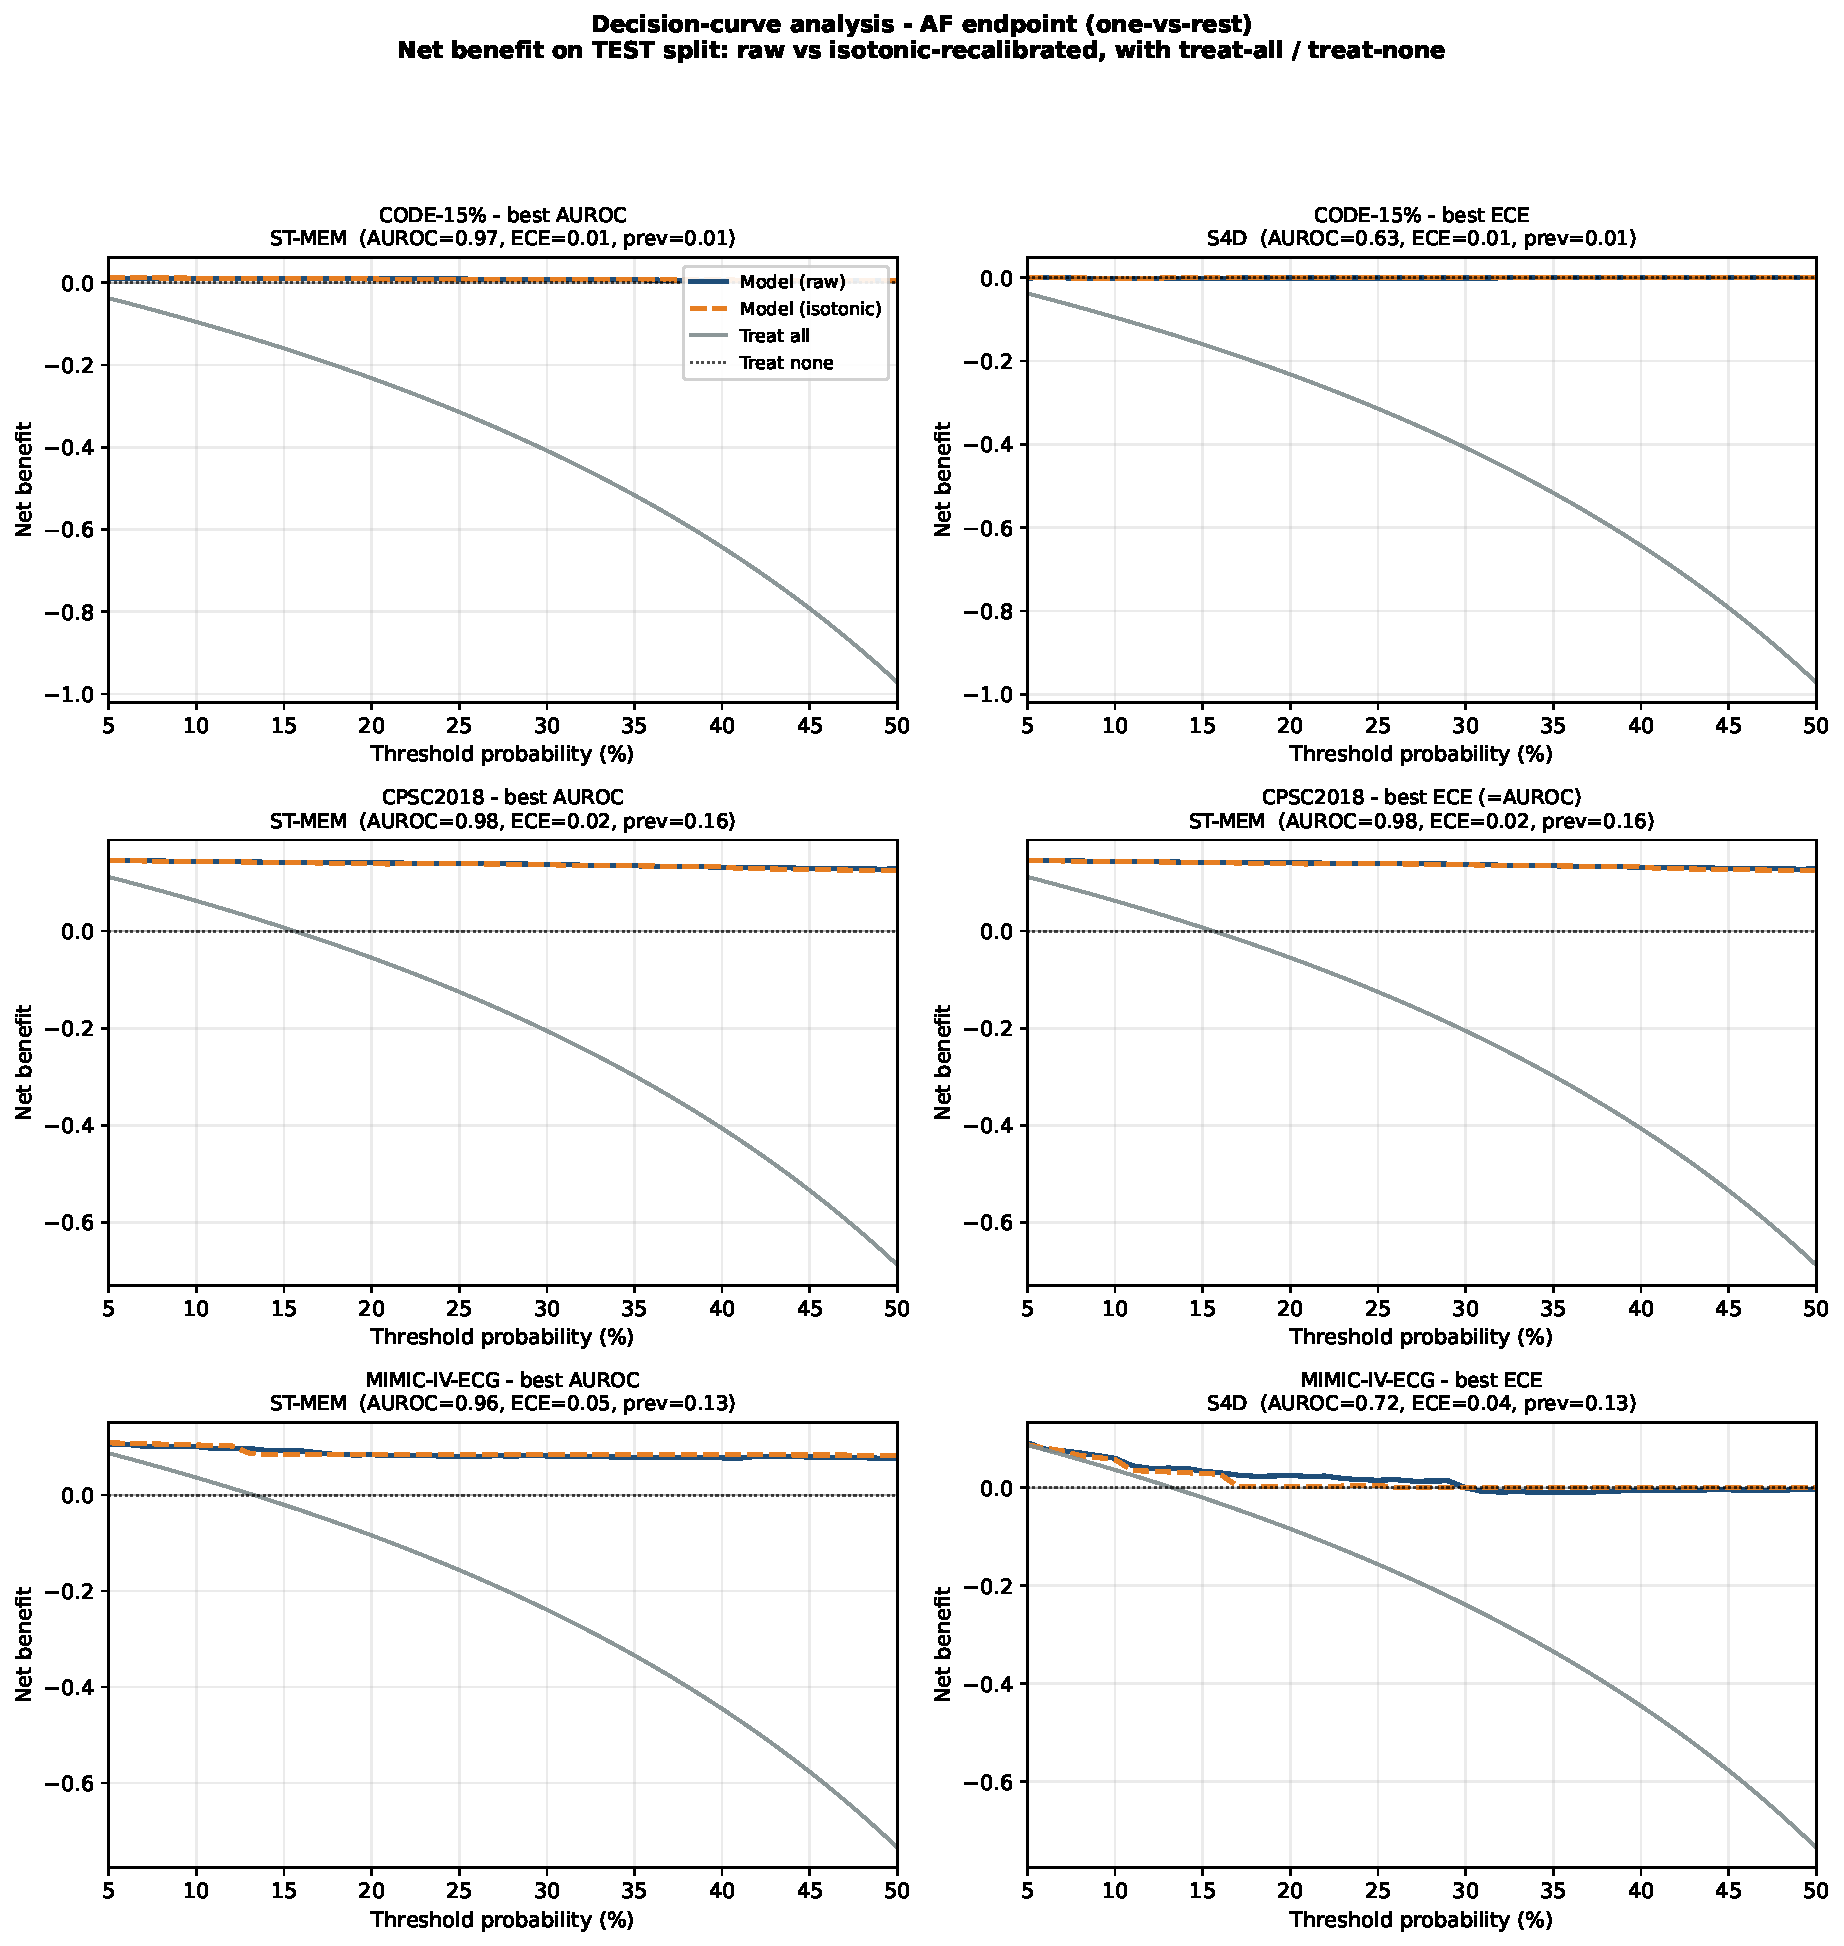
\includegraphics[width=0.96\linewidth]{figures/fig_dca_af.pdf}
  \caption{Decision-curve analysis for AF on CODE-15\%, CPSC2018, and MIMIC-IV-ECG.}
  \label{fig:dca-af}
\end{figure}

\subsection{Multi-Seed Robustness}
\label{sec:extended-robustness}

To show the headline conclusions are not split artefacts, we re-run the PTB-XL and
MIMIC-IV-ECG cells over 10 patient-level resplits (seeds 0--9; Table~\ref{tab:robustness},
Figure~\ref{fig:robustness}). The PTB-XL discrimination--calibration tradeoff is fully robust:
S4D has the lowest macro ECE of all six encoders in \textbf{10/10} seeds (mean gap $0.045$).
The within-domain finding is partially robust: ECG-FM trails MERL and ST-MEM in every seed,
but its AUROC ($0.792\pm0.015$) is \emph{statistically tied} with the supervised S4D baseline
($0.777\pm0.019$)---so we claim only that within-domain pretraining fails to beat the strong
self-supervised models, not that it underperforms a supervised baseline.

\begin{table}[t]
\centering
\caption{Multi-seed robustness (10 patient-level resplits, seeds 0--9): mean$\pm$std macro AUROC and ECE on the two multi-morbidity datasets. The PTB-XL discrimination--calibration tradeoff (S4D best-calibrated) holds in 10/10 seeds; ECG-FM trails MERL/ST-MEM on MIMIC in all seeds but is statistically tied with the S4D baseline.}
\label{tab:robustness}
\small
\begin{tabular}{llcc}
\toprule
Dataset & Model & AUROC (mean$\pm$std) & ECE (mean$\pm$std) \\
\midrule
  PTB-XL & MERL & 0.844$\pm$0.013 & 0.092$\pm$0.004 \\
   & ST-MEM & 0.852$\pm$0.015 & 0.119$\pm$0.009 \\
   & HuBERT-ECG & 0.801$\pm$0.018 & 0.141$\pm$0.009 \\
   & ECGFM-KED & 0.778$\pm$0.018 & 0.086$\pm$0.009 \\
   & ECG-FM & 0.812$\pm$0.015 & 0.100$\pm$0.010 \\
   & S4D & 0.785$\pm$0.021 & 0.062$\pm$0.004 \\
  \midrule
  MIMIC-IV-ECG & MERL & 0.882$\pm$0.012 & 0.063$\pm$0.004 \\
   & ST-MEM & 0.864$\pm$0.013 & 0.077$\pm$0.005 \\
   & HuBERT-ECG & 0.835$\pm$0.013 & 0.090$\pm$0.007 \\
   & ECGFM-KED & 0.744$\pm$0.018 & 0.066$\pm$0.006 \\
   & ECG-FM & 0.792$\pm$0.015 & 0.078$\pm$0.003 \\
   & S4D & 0.777$\pm$0.019 & 0.046$\pm$0.004 \\
\bottomrule
\end{tabular}
\end{table}

\begin{figure}[t]
  \centering
  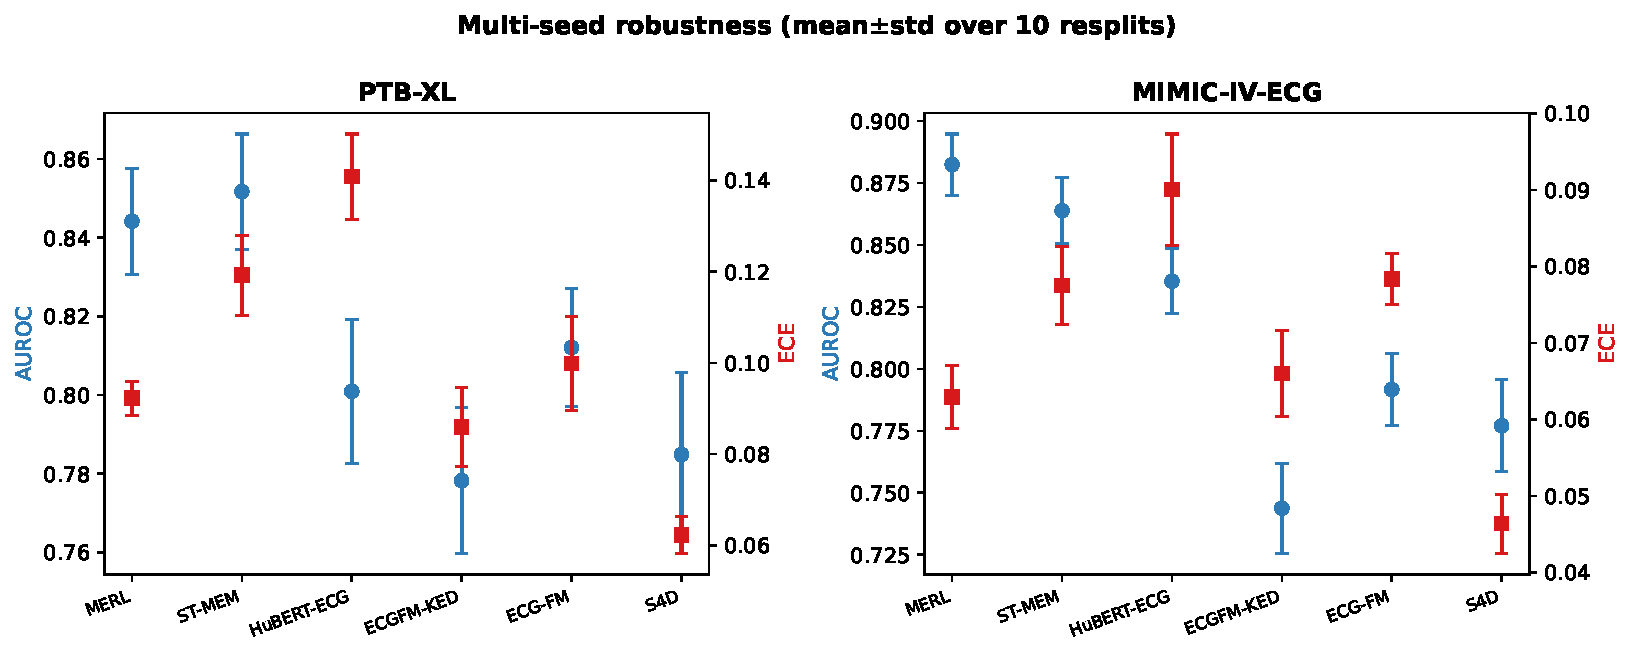
\includegraphics[width=0.96\linewidth]{figures/fig_robustness.pdf}
  \caption{Macro AUROC (blue) and ECE (red) as mean$\pm$std over 10 resplits, PTB-XL and
    MIMIC-IV-ECG. Rankings on both axes are stable.}
  \label{fig:robustness}
\end{figure}

\subsection{Mechanistic Regression: What Drives Miscalibration?}
\label{sec:extended-mechanistic}

To move beyond scatter plots we regress per-class ECE on candidate drivers across all
evaluated class-cells (OLS, $n{=}149$, $R^2{=}0.85$; Figure~\ref{fig:mechanistic}). Controlling
for everything else, \textbf{dataset/task structure dominates}: relative to PTB-XL, ECE is
lower by $0.074$ (CODE-15\%) and $0.076$ (CPSC2018) (both CIs exclude 0)---the multi-label
PTB-XL task is intrinsically harder to calibrate. \textbf{Masked-prediction pretraining}
independently raises ECE ($+0.044$ vs.\ contrastive, significant), while the
\textbf{supervised} objective lowers it ($-0.018$). At the class level, higher AUROC is
associated with slightly \emph{lower} ECE once dataset is controlled for---confirming that the
``rank well, calibrate poorly'' tradeoff is a model$\times$task phenomenon (the high-AUROC
foundation models on multi-label PTB-XL), not a universal law.

\begin{figure}[t]
  \centering
  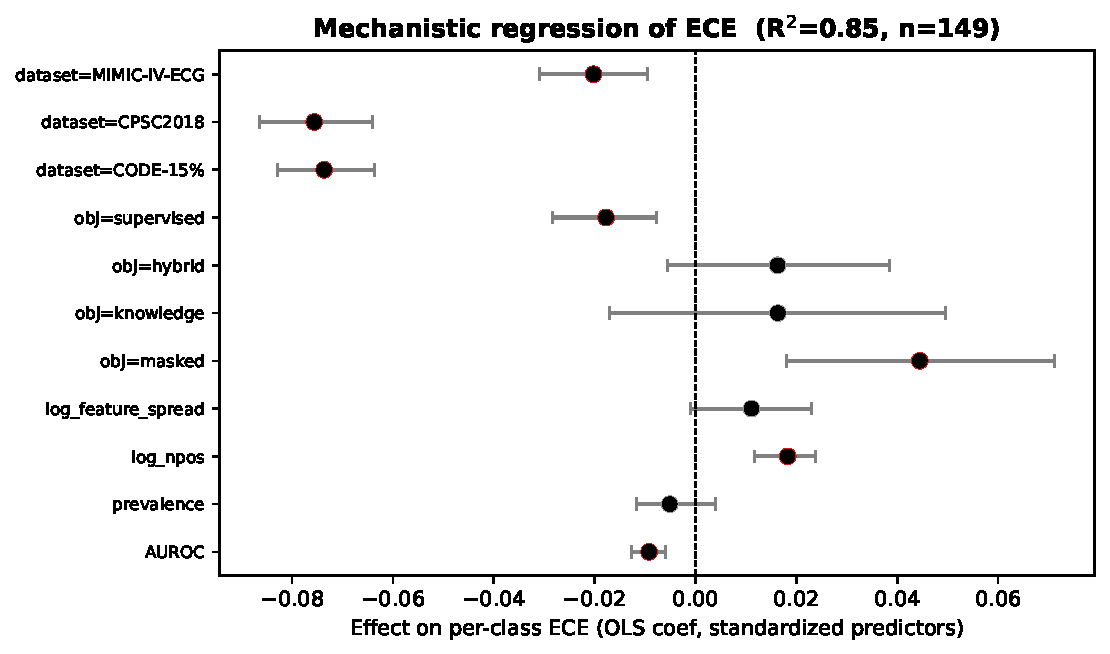
\includegraphics[width=0.82\linewidth]{figures/fig_mechanistic.pdf}
  \caption{OLS coefficients (standardized continuous predictors) for per-class ECE.
    Red = 95\% bootstrap CI excludes 0. Dataset and pretraining-objective effects dominate.}
  \label{fig:mechanistic}
\end{figure}

\subsection{Subgroup Calibration Across All Encoders}
\label{sec:extended-subgroup}

Extending the subgroup audit to all six encoders on PTB-XL (Figure~\ref{fig:subgroup-exp})
reveals a consistent age gradient: macro ECE rises from the $<$55 group to the $\geq$70 group
for \emph{every foundation model} (e.g.\ MERL $0.094\!\to\!0.143$, ST-MEM $0.111\!\to\!0.189$,
HuBERT-ECG $0.126\!\to\!0.183$), whereas the supervised S4D baseline stays flat
($0.117\!\to\!0.114$). Global calibration therefore hides a safety-relevant subgroup effect
specific to foundation-model representations: elderly patients receive the least reliable
probabilities from exactly the highest-AUROC models. This motivates subgroup-stratified
calibration auditing before deployment.

\begin{figure}[t]
  \centering
  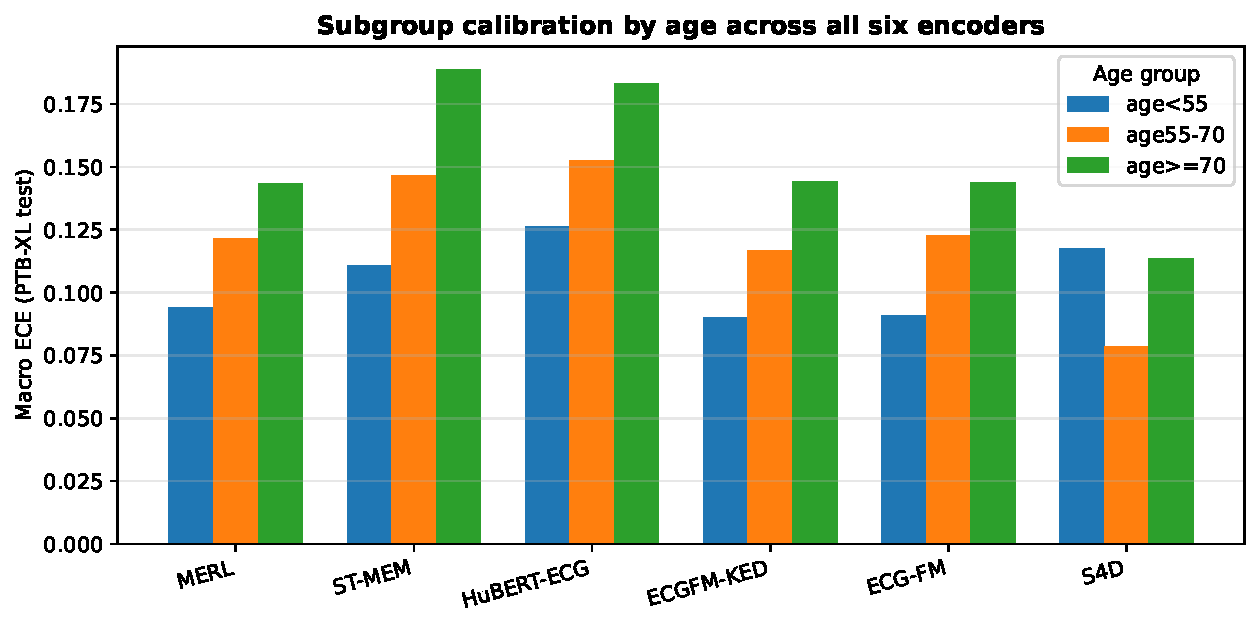
\includegraphics[width=0.92\linewidth]{figures/fig_subgroup_expanded.pdf}
  \caption{Macro ECE by age group across all six encoders (PTB-XL test). Foundation models
    degrade with age; the supervised baseline does not.}
  \label{fig:subgroup-exp}
\end{figure}
